\documentclass{article}
\usepackage{import}
\usepackage{amsmath}
\usepackage{tabularray}
\usepackage{float}


\import{lib/latex/}{wgmlgz}
\patchcmd{\thebibliography}{\section*}{\section}{}{}

\begin{document}
\itmo[
      variant=13,
      labn=2,
      discipline=Вычислительная математика,
      group=P3212,
      student=Соколов Анатолий Владимирович,
      teacher=Наумова Надежда Александровна 
]
\lstset{language=rust}
\newgeometry{
  a4paper,
  top=20mm,
  right=10mm,
  bottom=20mm,
  left=30mm
}
\tableofcontents

\section{Задание}
% \begin{enumerate}
      Вычислительная часть лабораторной работы должна быть представлена в виде таблиц и отображена только в отчете.
      \begin{enumerate}
            \item Отделить корни заданного нелинейного уравнения графически (вид уравнения представлен в табл. 2.6)
            \item График исследуемой функции отобразить в отчете
            \item Определить интервалы изоляции корней
            \item Уточнить корни заданного нелинейного уравнения с точностью $\varepsilon=10^{-2}$
            \item Используемые методы для уточнения каждого из трех корней многочлена представлены в табл. 2.7
            \item Вычисления оформить в виде таблиц (табл. 2.1–2.5), в зависимости от заданного метода. Для всех значений в таблицах удержать 3 знака после запятой;
      \end{enumerate}

\subsection{Вариант}

\subsection{Для нелинейных уравнений должно быть реализовано}

\begin{enumerate}
      \item Все численные методы (см. табл. 2.8) должны быть реализованы в виде класса /метода/функции;
      \item Пользователь выбирает уравнение, корень/корни которого требуется вычислить (3–5 функций, в том числе и трансцендентные), из тех, которые предлагает программа;
      \item Предусмотреть ввод исходных данных (границы интервала, погрешность вычисления) из файла или с клавиатуры по выбору конечного пользователя;
      \item Организовать вывод графика функции на исследуемом интервале (с запасом);
      \item Выполнить верификацию исходных данных. Необходимо анализировать наличие корня на введенном интервале. Если на интервале несколько корней или они отсутствуют – выдавать соответствующее сообщение. Программа должна реагировать на некорректные введенные данные;
      \item Для методов, требующих начальное приближение к корню (методы Ньютона, секущих, хорд с фиксированным концом, простой итерации), выбор начального приближения (а или b) вычислять в программе;
      \item Для метода простой итерации проверять достаточное условие сходимости метода на введенном интервале. Если оно не выполняется, выводить соответствующее сообщение. При этом попытаться решить нелинейное уравнение, ограничив итерационный процесс заданным в программе максимальным числом итераций;
      \item Для каждого метода учитывать все критерии выхода из итерационного цикла. Проверить, как изменятся результаты, если учитывать либо критерии по аргументу, либо критерии по функции;
      \item Предусмотреть вывод результатов (найденный корень уравнения, значение функции в корне, число итераций) в файл или на экран по выбору конечного пользователя;
      \item Проанализировать полученные результаты, оценить точность решения задачи;
      \item Программа должна быть протестирована на различных наборах данных, в том числе и некорректных.
\end{enumerate}

\subsection{Для систем нелинейных уравнений должно быть реализовано}

\begin{enumerate}
      \item Пользователь выбирает предлагаемые программой системы двух нелинейных уравнений (2–3 системы);
      \item Организовать вывод графика функций.
      \item Ввести начальные приближения с клавиатуры;
      \item Для метода простой итерации проверить достаточное условие сходимости. Если оно не выполняется, выводить соответствующее сообщение. При этом попытаться решить систему нелинейных уравнений, ограничив итерационный процесс заданным в программе максимальным числом итераций;
      \item Организовать вывод вектора неизвестных: ;
      \item Организовать вывод количества итераций, за которое было найдено решение;
      \item Организовать вывод вектора погрешностей: ;
      \item Проверить правильность решения системы нелинейных уравнений.
      \item Программа должна быть протестирована при различных наборах данных, в том числе и некорректных.
\end{enumerate}

\subsection{Варианты задания}
\textbf{Выбор метода для вычислительной реализации задачи}
      \\
      $$x^3+4.81x^2-17.37x+5.38$$
      Метод простой итерации
      \\
      $$\begin{cases}
            &\sin y + 2x=2\\
            &y+\cos(x-1)=0.7
      \end{cases}$$
      \textbf{Выбор метода для программной реализации задачи}
      \\
      Решение нелинейных уравнений: метод половинного деления, метод секущих, метод простой итерации
      \\
      Решение систем нелинейных уравнений: метод Ньютона.
\subsection{Цель работы}
      Изучить численные методы решения нелинейных уравнений и их систем, найти корни заданного нелинейного уравнения/системы нелинейных уравнений, выполнить программную реализацию методов.

\section{Выполнение}
      $$x_3(2.138,0)$$
      $$x_2(0.345,0)$$
      $$x_1(-7.293,0)$$
      \begin{table}[H]
            \centering
            \begin{tabular}{|*{4}{c|}}
            \hline
            Номер & Крайний & Крайний & Центральный  \\
            варианта & правый корень & левый корень & корень \\
            \hline
            13 & Метод простой итерации (5) & Метод хорд (2) & Метод Ньютона (3) \\
            \hline
            \end{tabular}
            \caption{Методы для вычислительной реализации}
      \end{table}
      \subsection{Рабочие формулы}
            Метод Ньютона $x_i=x_{i-1}-\frac{f(x_{i-1})}{f'(x_{i-1})}$ \\
            Метод половинного деления $x_i=\frac{x_{i-1}+x_{i+1}}{2}$ \\
            Метод простой итерации $x_{i+1}=\varphi(x_i)$, где $\varphi(x)=x$ ($x$ выражается из исходной функции $f(x))$\\
            Метод хорд $x_{i+1}=\frac{a_i f(b_i)-b_i f(a_i)}{f(b_i)-f(a_i)}$
      
      \subsection{Графики функций}
            \begin{figure}[H] 
                  \begin{center}  
                        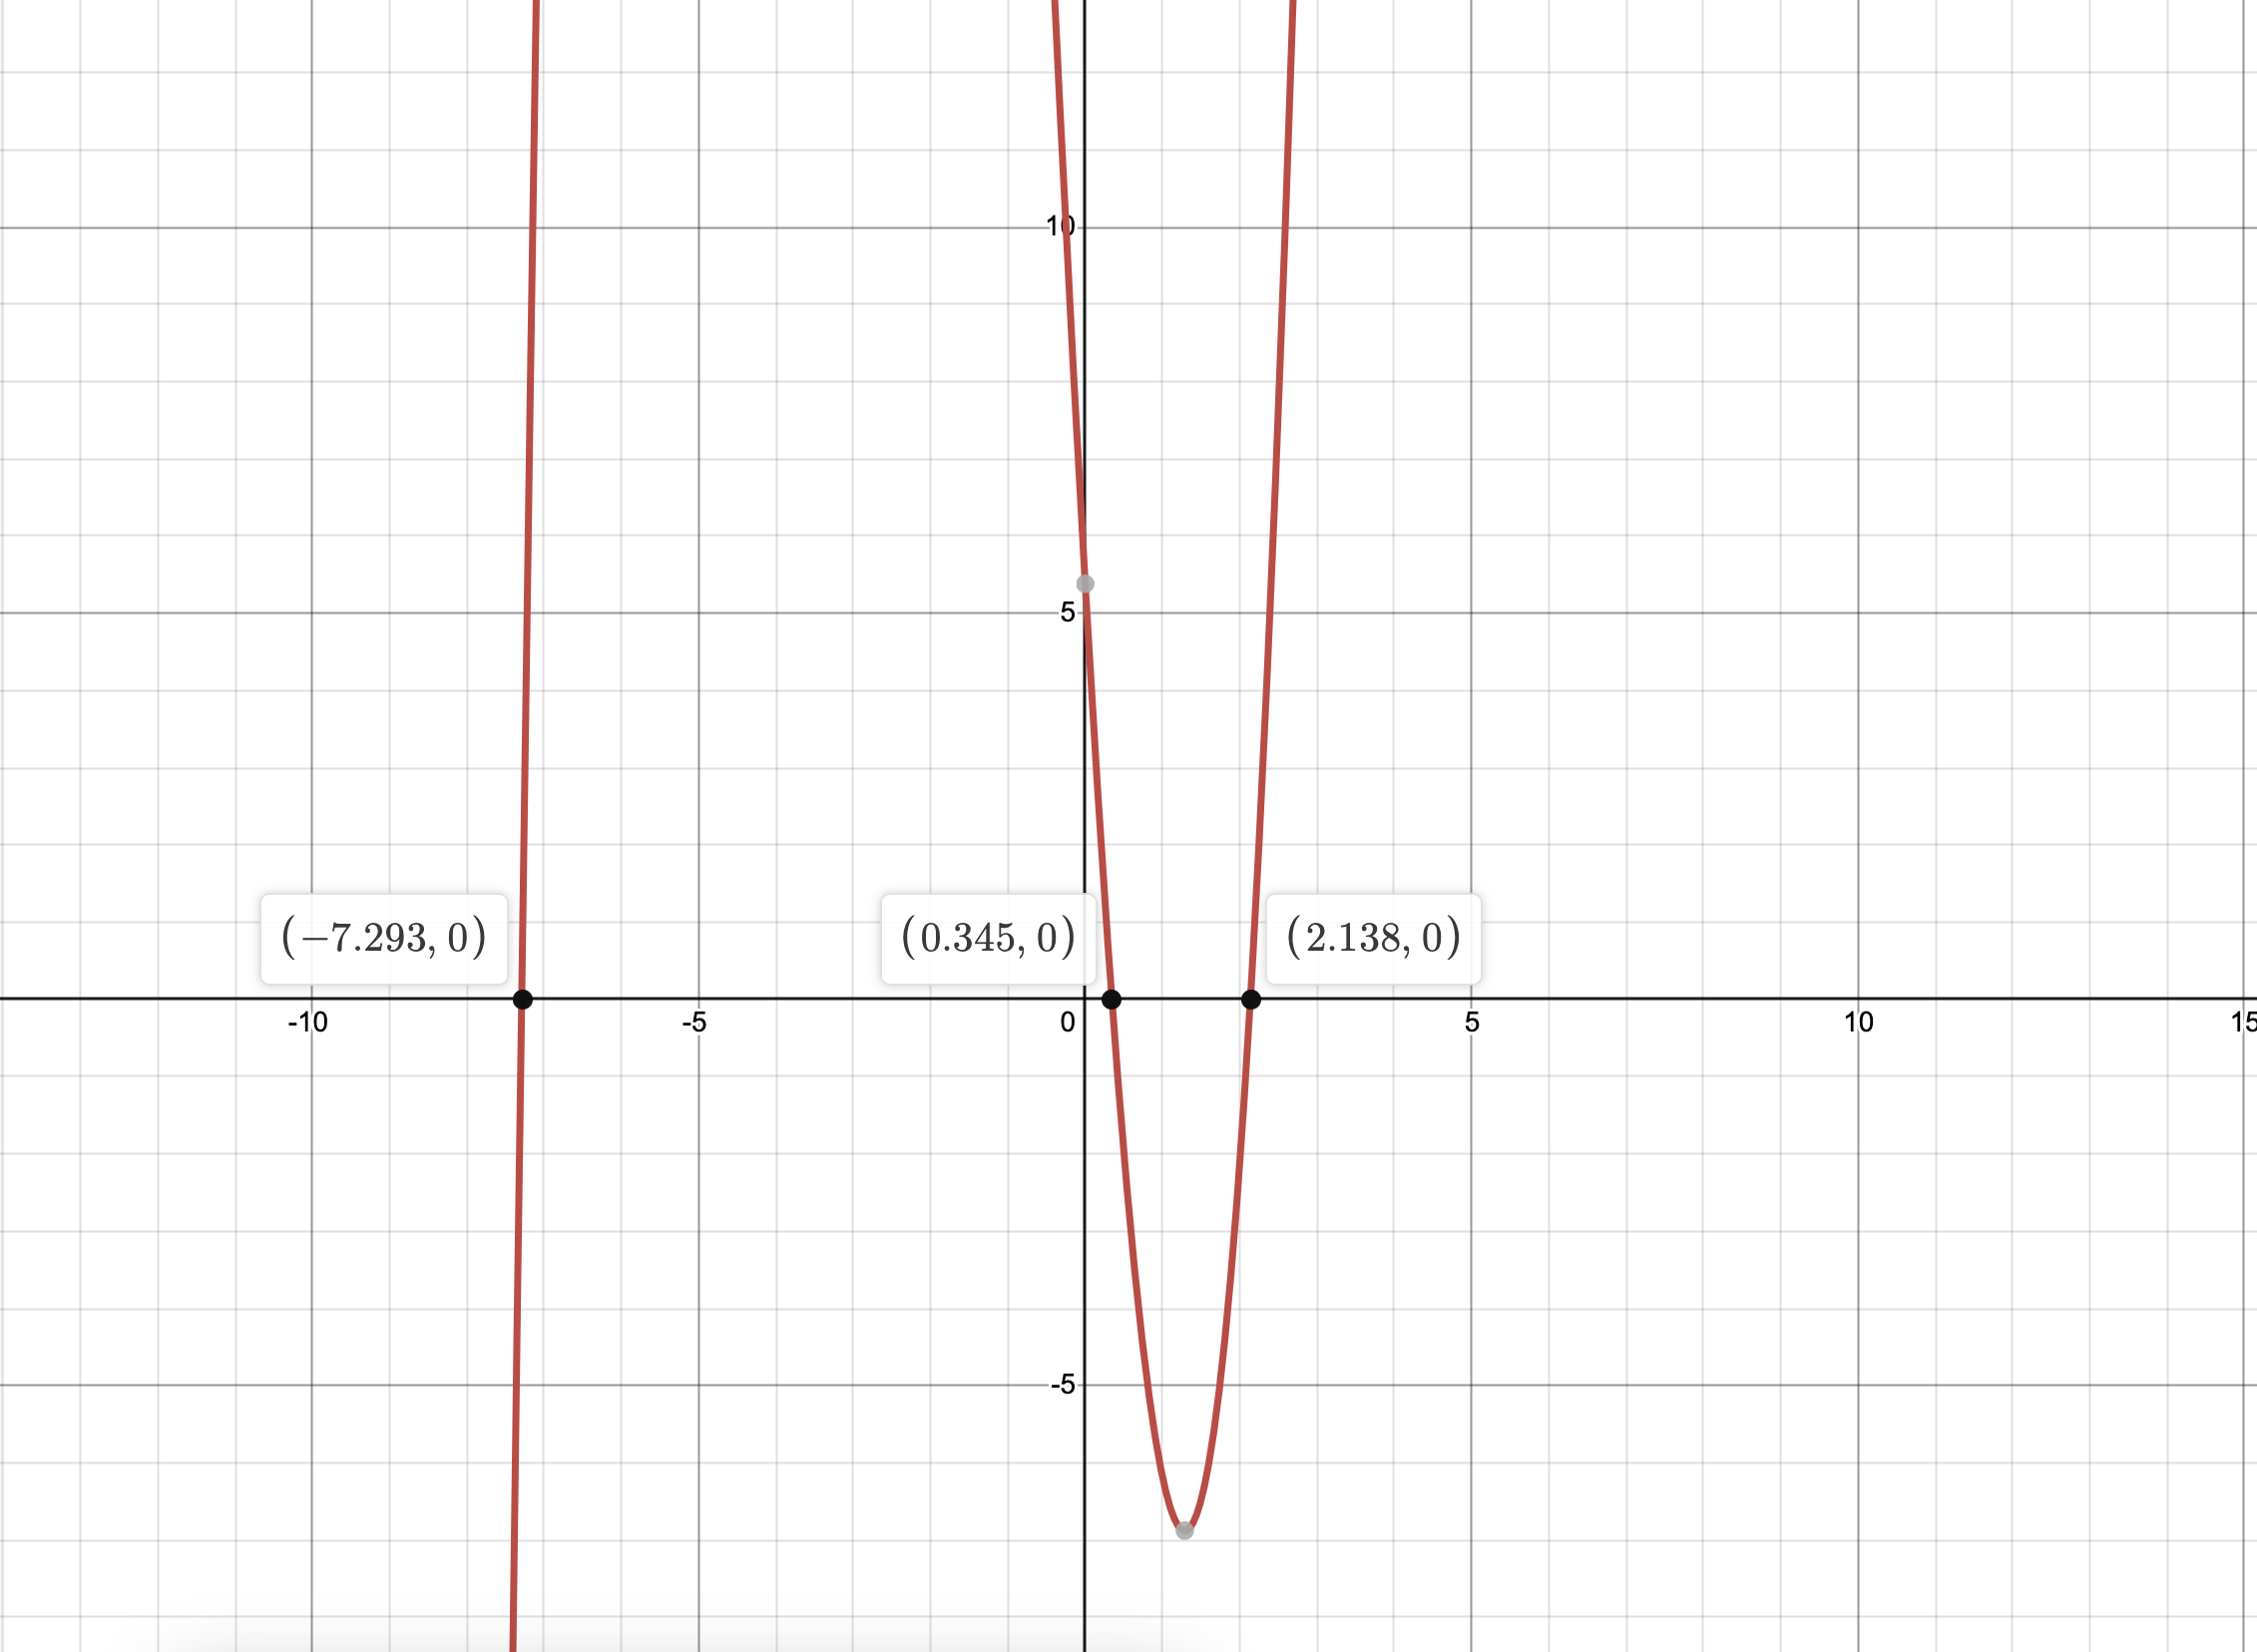
\includegraphics[scale=0.4]{graph.png}
                        \caption{\small \sl  $x^3+4.81x^2-17.37x+5.38$}  
                  \end{center}  
            \end{figure}

            \begin{figure}[H] 
                  \begin{center}  
                        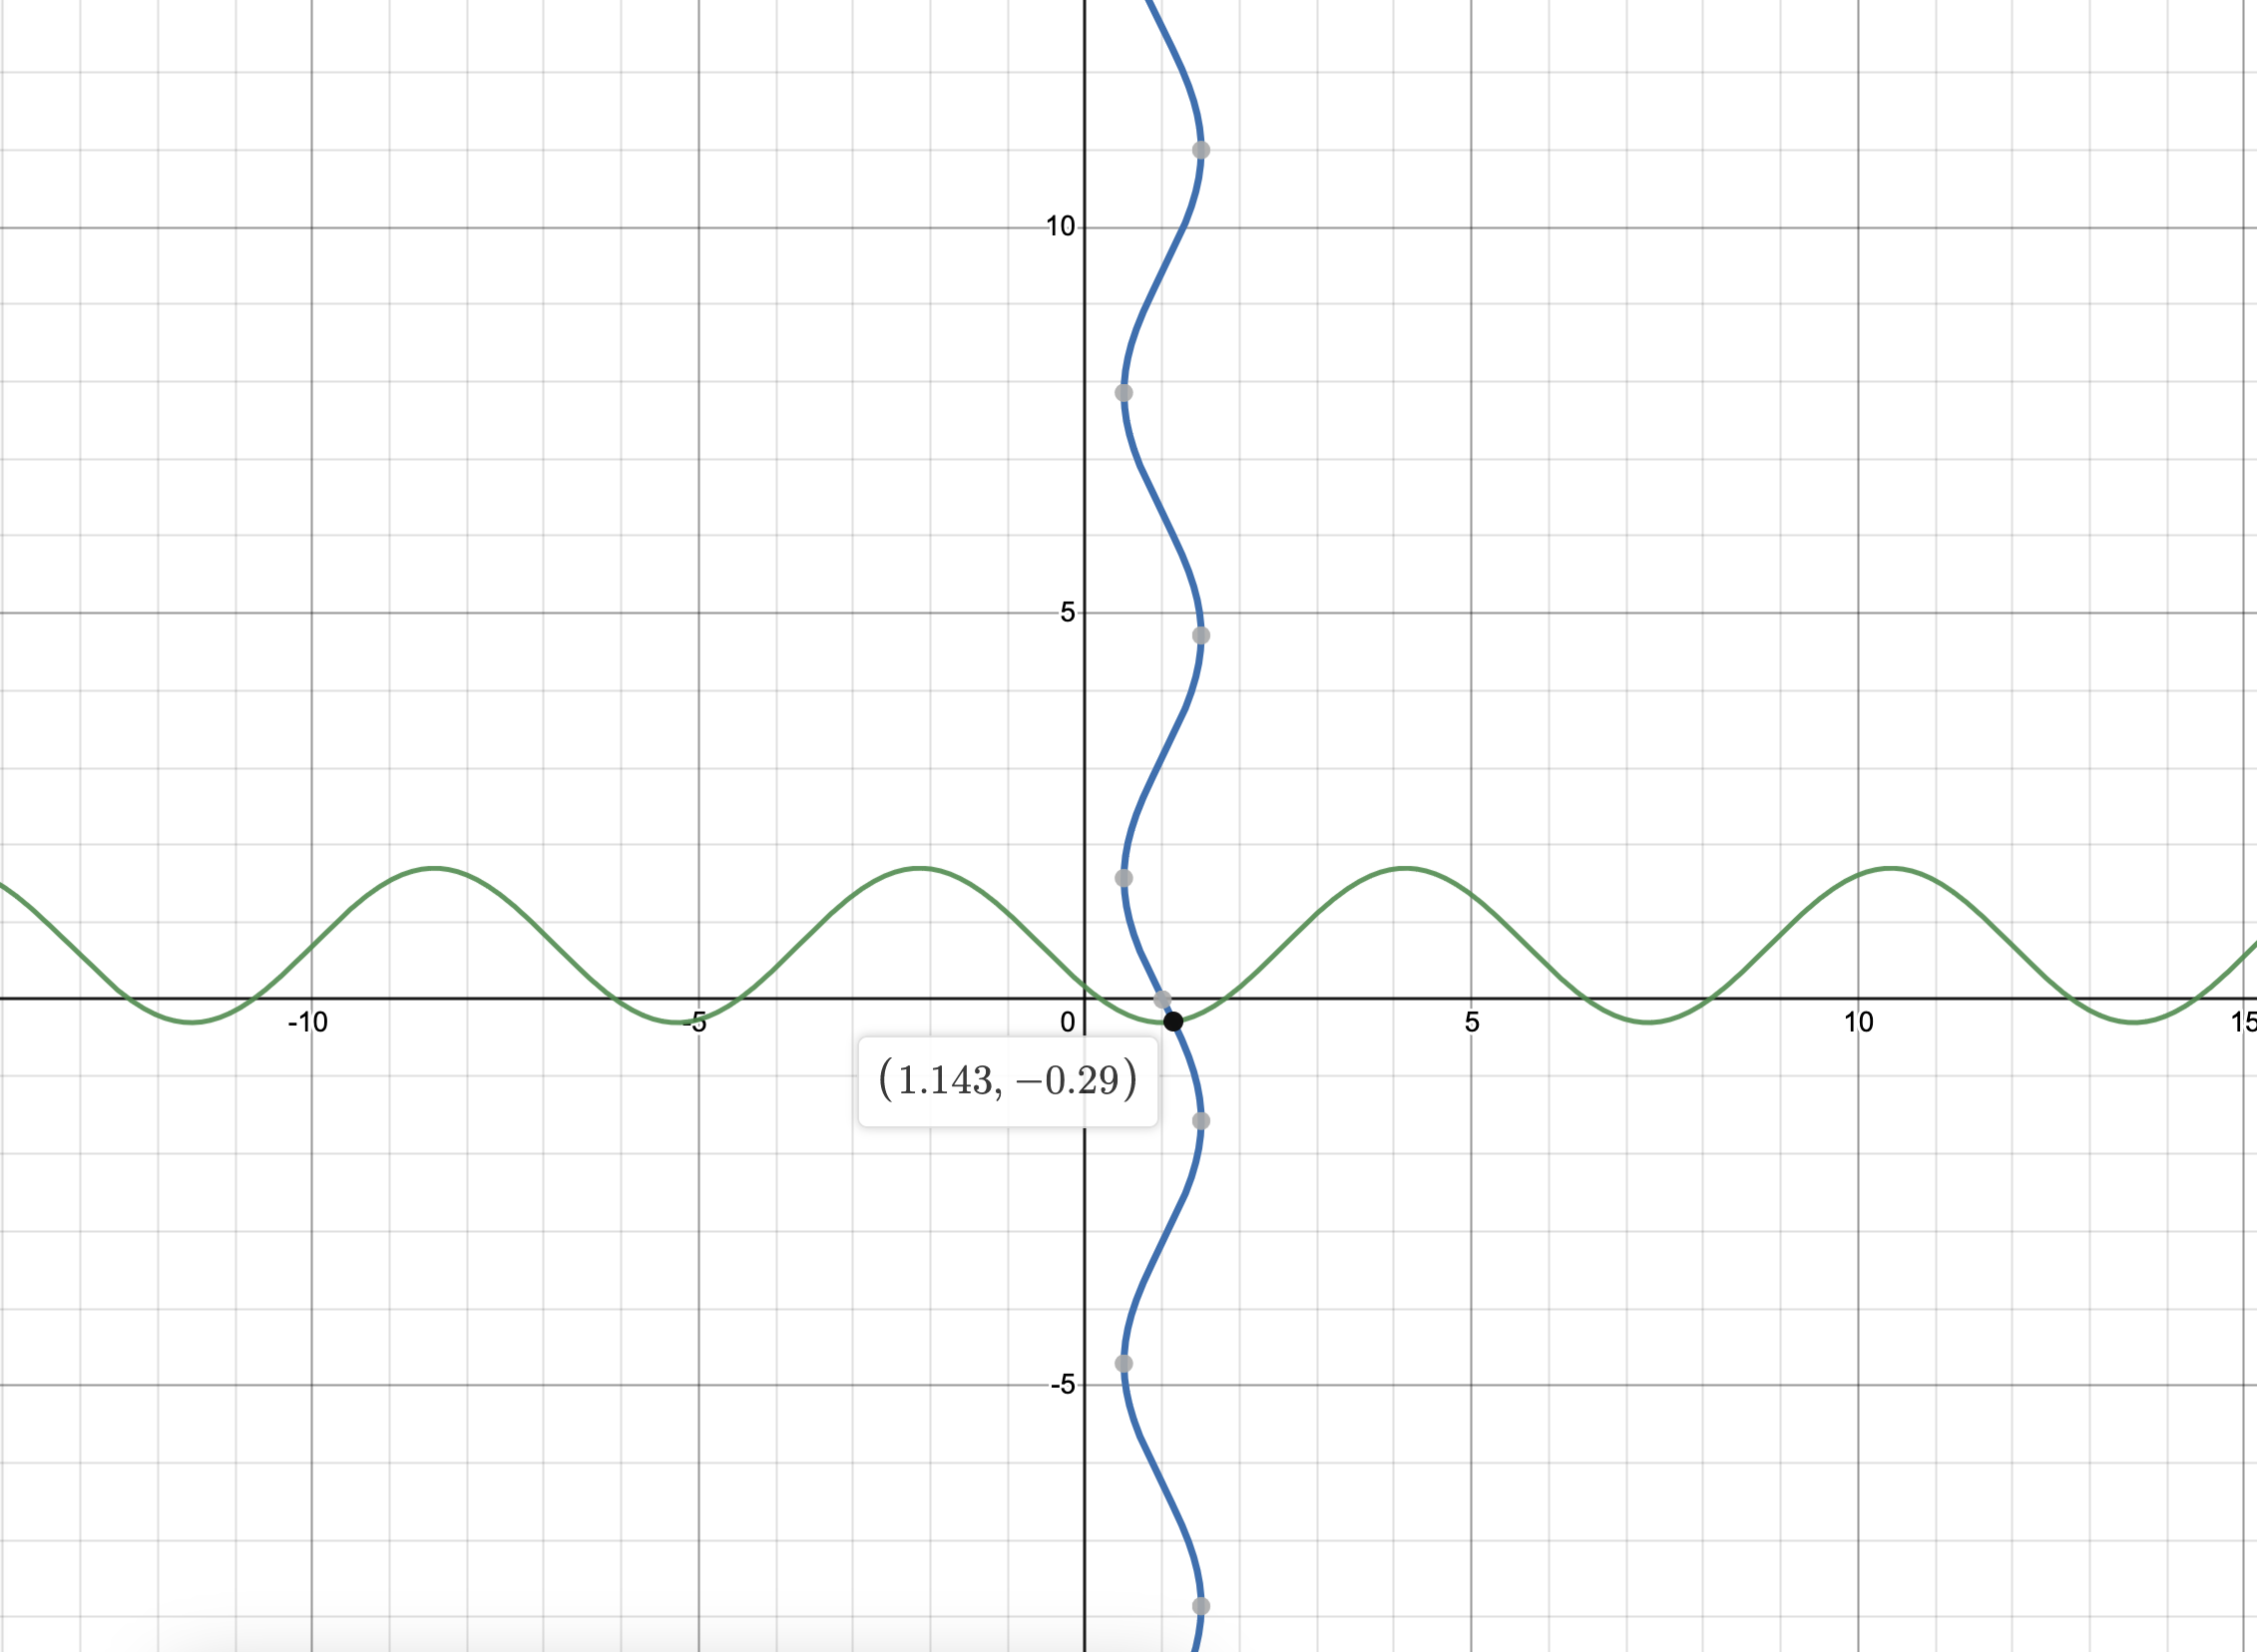
\includegraphics[scale=0.4]{graph2.png}
                        \caption{\small \sl  $\begin{cases}
                              &\sin y + 2x=2\\
                              &y+\cos(x-1)=0.7
                        \end{cases}$}  
                  \end{center}  
            \end{figure}

      \subsection{Метод простой итерации для $x_3$}

            Приведём уравнение:
            \[
            x^3+4.81x^2-17.37x+5.38
            \]
            \\
            Решим через параметр $\lambda$:
            Пусть начальное приближение будет:
            \[    
            a_0 = 1.4;\ b_0 = 1.9\]
            \[
            f(x) = x^3+4.81x^2-17.37x+5.38 \]
            \[\lambda f(x) = 0\ (\lambda!=0)\]
            \[\varphi(x)\ = x+ \lambda f(x) \]
            \[\varphi'(x)\ = 1+ \lambda f'(x) \]
            \[f'(x) =-17.37 + 9.62 x + 3 x^2\]
            \[f'(1.4) = -17.37 + 9.62 \cdot 1.4 + 3\cdot(1.4)^2=1.978\]
            \[f'(2.2) = -17.37 + 9.62 \cdot 2.2 + 3\cdot(2.2)^2=18.314\]
            Так как $f'[a, b] > 0$, то рассматриваем:
            \[
            \lambda = - \frac{1}{max|f'(x)|} = -\frac{1}{18.314} = 0.054\] 
            Подставим:
            \[\varphi(x) = x+(-1/(-17.37 + 9.62 * 2.2 + 3 * (2.2)^2))*(x^3+4.81x^2-17.37x+5.38) \] 
            \[= -0.293764 + 1.94845 \cdot x - 0.262641 \cdot x^2 - 0.054603 \cdot x^3 \]
            \[\varphi'(x) = 1.94845 - 0.525282 * x - 0.163809*x^2 \]
            Проверим точки:
            \[\varphi'(1.4) = 1.94845 - 0.525282 * 1.4 - 0.163809*1.4^2 < 1\]
            \[\varphi'(2.2) = 1.94845 - 0.525282 * 2.2 - 0.163809*2.2^2  < 1\]
            Условие сходимости выполняется!
            \[x_0 = 1.4 \]
            \[x_1 = \varphi(x_0) = -0.293764 + 1.94845 \cdot (1.4) - 0.262641 \cdot (1.4)^2 - 0.054603 \cdot (1.4)^3 = 1.769459008\]
            \[x_2 = -0.293764 + 1.94845 \cdot (1.769459008) - 0.262641 \cdot (1.769459008)^2 - 0.054603 \cdot (1.769459008)^3 = 2.0291045184565837\] 
            \[f(x_2) = (1.769459008)^3+4.81 \cdot (1.769459008)^2-17.37 \cdot (1.769459008)+5.38 = -4.755314315965413\]
            $$\dots$$
            \[
            f(x) = x^3+4.81x^2-17.37x+5.38 \]
            \[\varphi(x)=  -0.293764 + 1.94845 \cdot x - 0.262641 \cdot x^2 - 0.054603 \cdot x^3 \]


            \begin{table}[h]
            \centering
                  \begin{tabular}{|*{6}{c|}}
                        \hline
                        Номер & $x_i$ & $x_{i+1}$ & $\varphi(x_{i+1})$& $f(x_{i+1})$& $|x_{i+1} - x_i|$  \\ \hline
                        0 & 1.4        & 1.76945901 & 2.02910452 & -1.7071388 & 0.36945901 \\  \hline
                        1 & 1.76945901 & 2.02910452 & 2.12230887 & -0.2600345 & 0.25964551 \\ \hline
                        2 & 2.02910452 & 2.12230887 & 2.13649639 & -0.0228481 & 0.09320435 \\ \hline
                        3 & 2.12230887 & 2.13649639 & 2.13773272 & -0.0019654 & 0.01418751 \\ \hline
                        4 & 2.13649639 & 2.13773272 & 2.13782878 & -0.0003413 & 0.00123633 \\ \hline
                  \end{tabular}
            \caption{Уточнение корня уравнения методом простой итерации}
            \end{table}

      \subsection{Метод хорд для $x_1$}
            Возьму за изолированный интервал $[-8, -7]$
            $$x^3+4.81x^2-17.37x+5.38$$
            Вычисление будем производить по формуле:
            \[
            x_i = \frac{a_if(b_i) - b_if(a_i)}{f(b_i) - f(a_i)}
            \]
            \begin{table}[H]
            \centering
                  \begin{tabular}{|*{8}{c|}}
                        \hline
                        Номер & $a$ & $b$ & $x$& $f(a)$& $f(b)$& $f(x)$& $|x_{i+1} - x_i|$  \\
                        \hline
                        0 & -8 & -7         & -7.2473578 & -59.82 & 19.66      & 3.24634659 & 0.24735783 \\ \hline
                        1 & -8 & -7.2473578 & -7.2861002 & -59.82 & 3.24634659 & 0.49019797 & 0.03874233 \\ \hline
                        2 & -8 & -7.2861002 & -7.2919027 & -59.82 & 0.49019797 & 0.07300449 & 0.00580254 \\ \hline
                        3 & -8 & -7.2919027 & -7.2927658 & -59.82 & 0.07300449 & 0.01085004 & 0.00086311 \\ \hline
                  \end{tabular}
            \caption{Уточнение корня уравнения методом хорд}
            \end{table}
            Тогда ответ:
            \[x \approx -7.2927658\]

      \subsection{Метод Ньютона для $x_2$}
                  Возьму за изолированный интервал $[0.3, 0.4]$
                  $$x^3+4.81x^2-17.37x+5.38$$
                  Вычисление будем производить по формуле:
                  \[
                  f(0.3)=0.3^3+4.81*0.3^2-17.37*0.3+5.38=0.6289
                  \]
                  \[
                  f(0.4)=0.4^3+4.81*0.4^2-17.37*0.4+5.38=-0.7344
                  \]
                  Найдем производные:
                  \[
                  f'(x)= -17.37 + 9.62 x + 3 x^2
                  \]
                  \[
                  f'(0.3)= -17.37 + 9.62 * 0.3 + 3 * 0.3^2 = -14.214
                  \]
                  \[
                  f'(0.4)= -17.37 + 9.62 * 0.4 + 3 * 0.4^2 = -13.042
                  \]
                  Первая производная сохраняет знаки \\
                  Найдем вторую производную
                  \[
                  f''(x)=9.62 + 6 x \\ 
                  f''(0.3)=9.62 + 6 * 0.3 = 11.42 \\
                  f''(0.4)=9.62 + 6 * 0.4 = 12.02    
                  \]
                  Вторая производная сохраняет знаки \\
                  Выполняется условие $f(a_0)\cdot f''(a_0)>0$, тогда $x_0 = a_0 = 0.3$
                  \begin{table}[H]
                        \centering
                              \begin{tabular}{|*{6}{c|}}
                              \hline
                              Номер & $x_i$ & $f(x_i)$ & $f'(x_i)$& $x_{i+1}$& $|x_{i+1}-x_i|$ \\ \hline
                              0 & 0.3        & 0.34424511 & 0.6289     & 20.526     & 0.04424511 \\ \hline
                              1 & 0.34424511 & 0.34506718 & 0.01126468 & 21.0371521 & 0.00082207 \\ \hline
                              2 & 0.34506718 & 0.34506747 & 3.9491E-06 & 21.0467603 & 2.8839E-07 \\ \hline
                              \end{tabular}
                  \caption{Уточнение корня уравнения методом Ньютона}
                  \end{table}

                  Условие окончания итер метода соблюдается: 
                  \[|x_n - x_{n-1}|\leq\varepsilon \ \ |f(x_n)|\leq\varepsilon\]
                  Тогда ответ:
                  \[x \approx 0.34506747\]

      \subsection{Решение системы нелинейных уравнений}

            $$\begin{cases}
                  &\sin y + 2x=2\\
                  &y+\cos(x-1)=0.7
            \end{cases}$$

            Определяем, что решение системы уравнений находится в квадрате:
            $$1\leqslant x\leqslant 2$$
            $$-1\leqslant y\leqslant 0$$

            $$\begin{cases}
                  &x=\frac{\left(2-\sin y\right)}{2}\\
                  &y=0.7-\cos(x-1)
            \end{cases}$$

            $$\frac{\partial x}{\partial x}=0$$
            $$\frac{\partial x}{\partial y}=\frac{\left(2-\sin y\right)}{2}$$

            $$\frac{\partial y}{\partial y}=0$$
            $$\frac{\partial y}{\partial x}=-\cos(x-1)$$

            $$\bigg| \frac{\partial x}{\partial x} \bigg| + \bigg| \frac{\partial x}{\partial y} \bigg| = \bigg| \frac{\left(2-\sin y\right)}{2} \bigg| \leqslant 1 $$
            $$\bigg| \frac{\partial y}{\partial x} \bigg| + \bigg| \frac{\partial y}{\partial y} \bigg| = | \cos(x-1) | \leqslant 1$$

            $$\max_{[x \in G]} |\varphi'| < 1 \rightarrow \text{Процесс сходящийся}$$ 
            \begin{table}[H]
                  \centering
                  \begin{tabular}{|c|c|c|c|c|c|c|}
                        \hline
                        \text{Номер итерации} & $x_i$ & $y_i$ & $x_{i+1}$ & $y_{i+1}$ & $|x_{i+1}-x_i|$ & $|y_{i+1}-y_i|$ \\ \hline
                        0 & 0 & 0 & 1 & 0.1597 & 1 & 0.1597 \\ \hline
                        1 & 1 & 0.1597 & 0.9205 & -0.3 & 0.0795 & 0.4597 \\ \hline
                        2 & 0.9205 & -0.3 & 1.1478 & -0.2968 & 0.2273 & 0.0032 \\ \hline
                        3 & 1.1478 & -0.2968 & 1.1463 & -0.2891 & 0.0015 & 0.0077 \\ \hline
                  \end{tabular}
                  \caption{Уточнение корня уравнения методом простой итерации}
            \end{table}

      \subsection{Блок-схема реализованного алгоритма}
            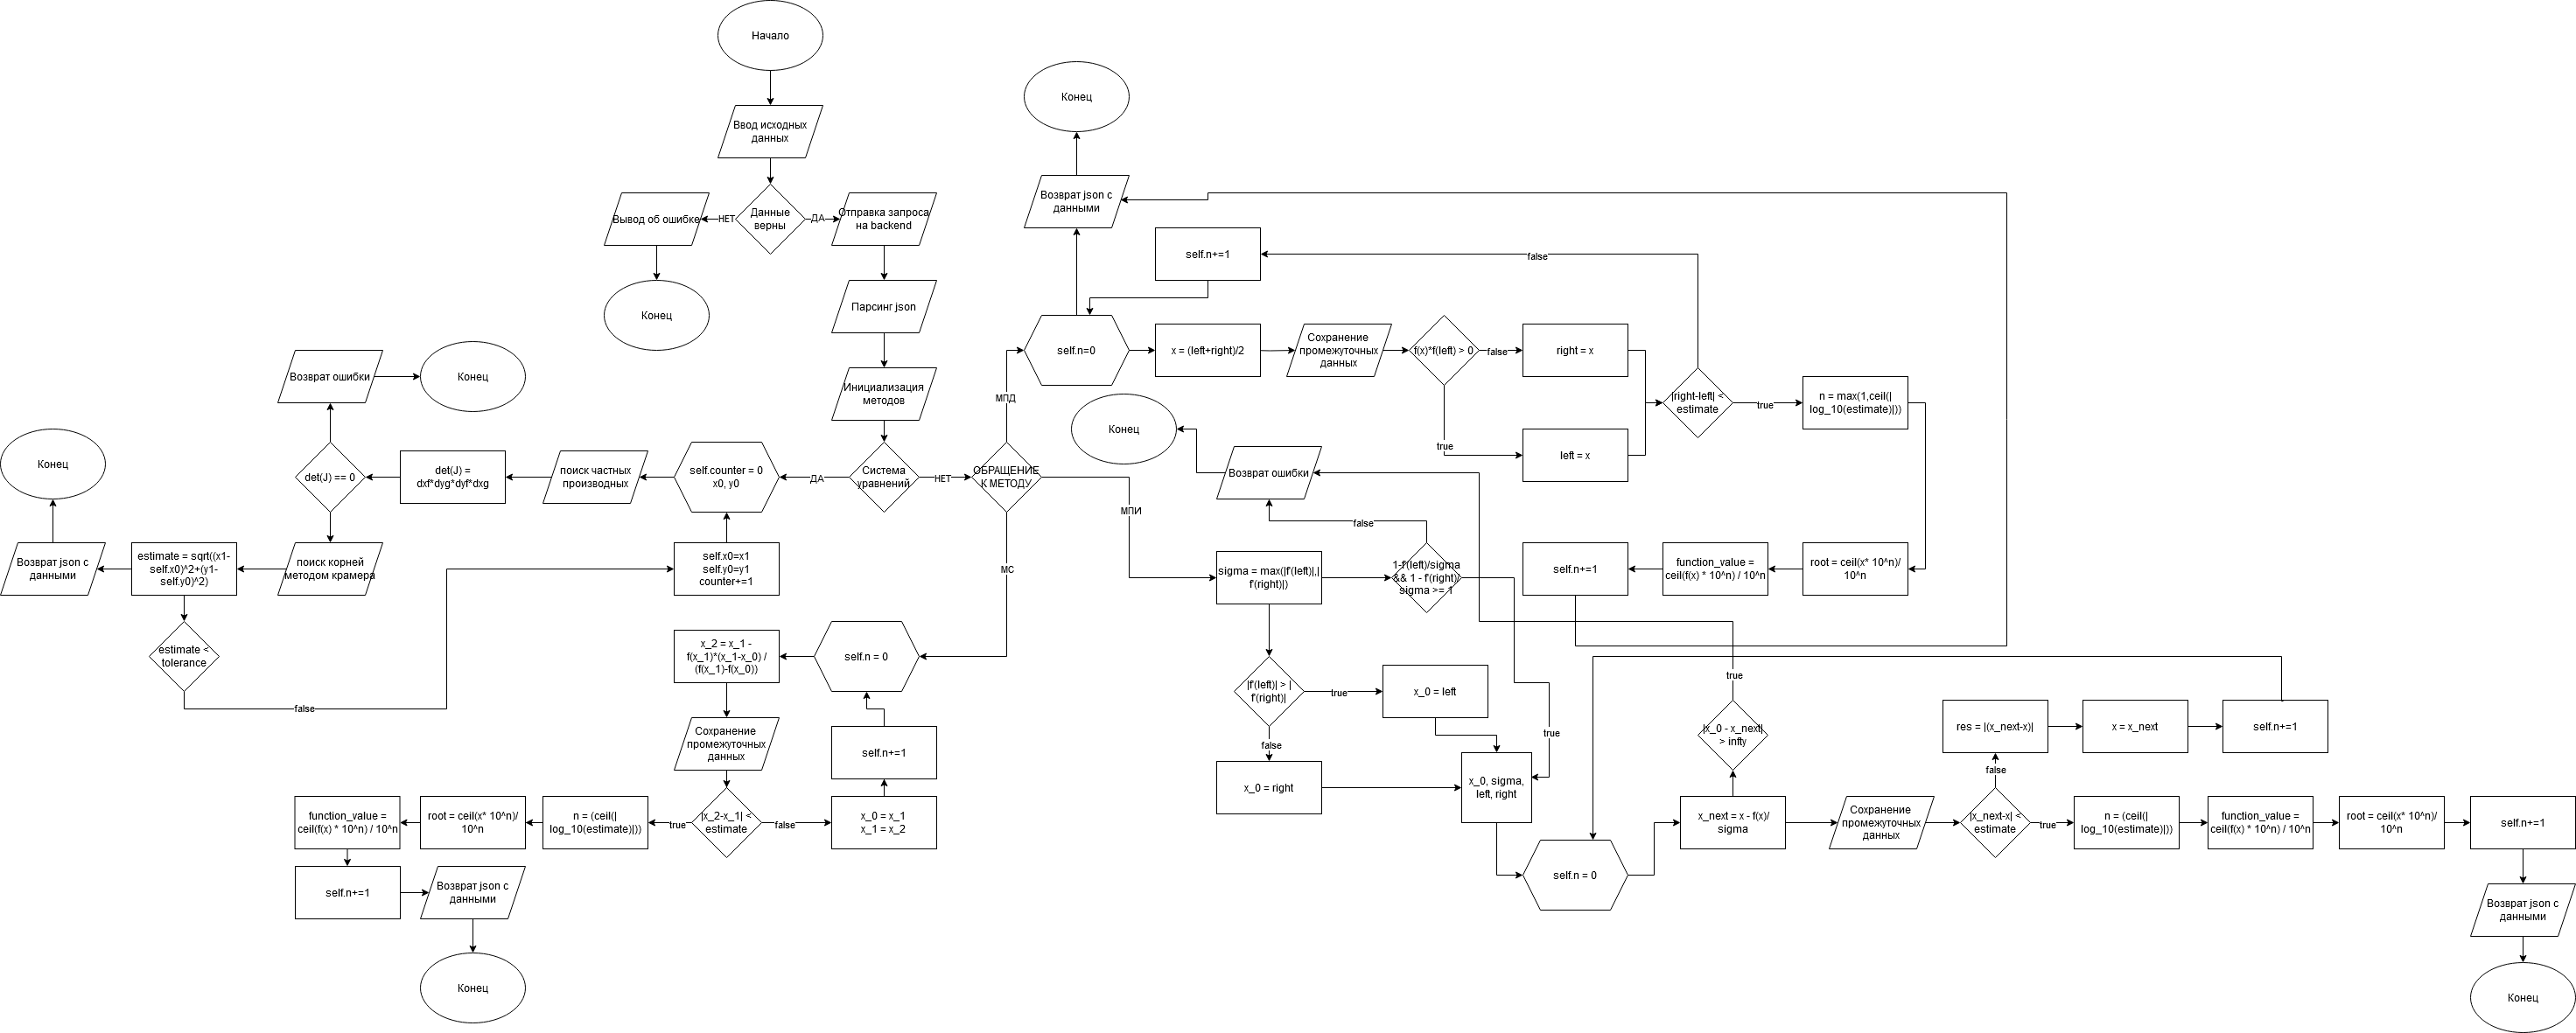
\includegraphics[scale=0.15]{НУиСНУ.png}
      \subsection{Ссылка на GitHub c основной реализацией}
            \href{https://github.com/isofinly/compmath}{Github}

      \subsection{Примеры и результаты работы программы}
            \begin{figure}[H] 
                  \begin{center}  
                        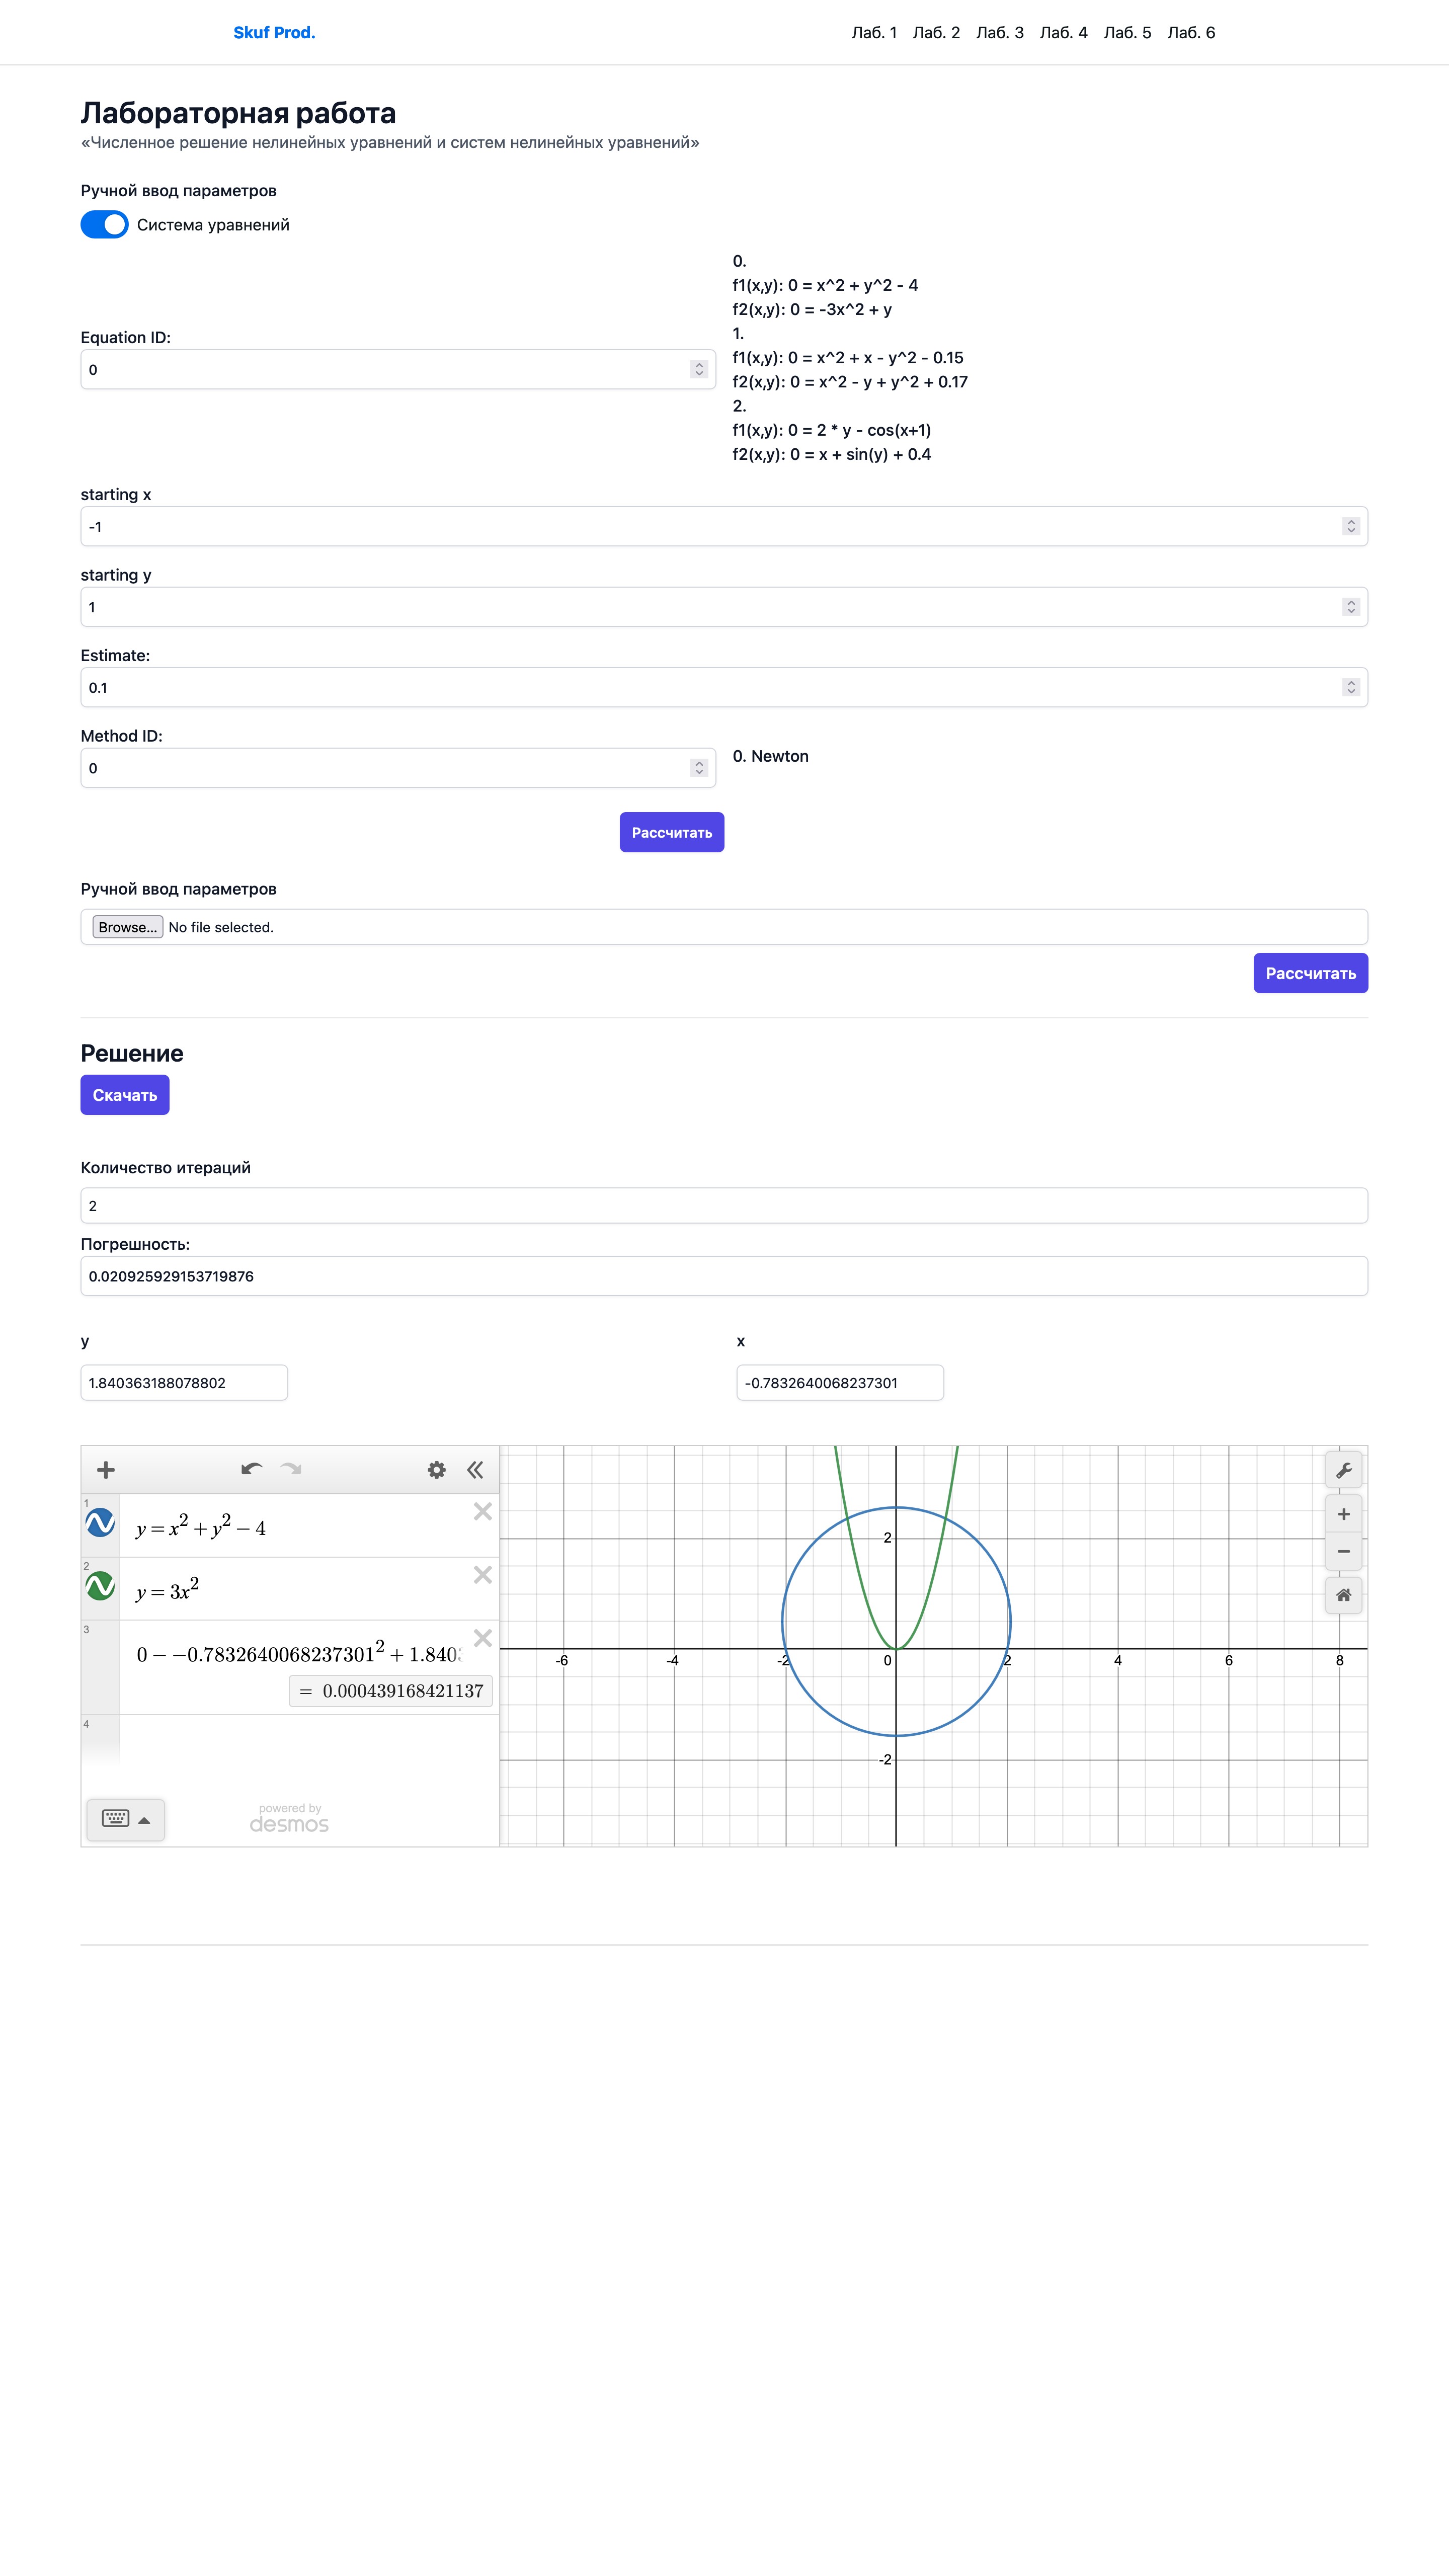
\includegraphics[scale=0.1]{SS1.png}
                        \caption{\small \sl UI 1}  
                  \end{center}  
            \end{figure}
            \begin{figure}[H] 
                  \begin{center}  
                        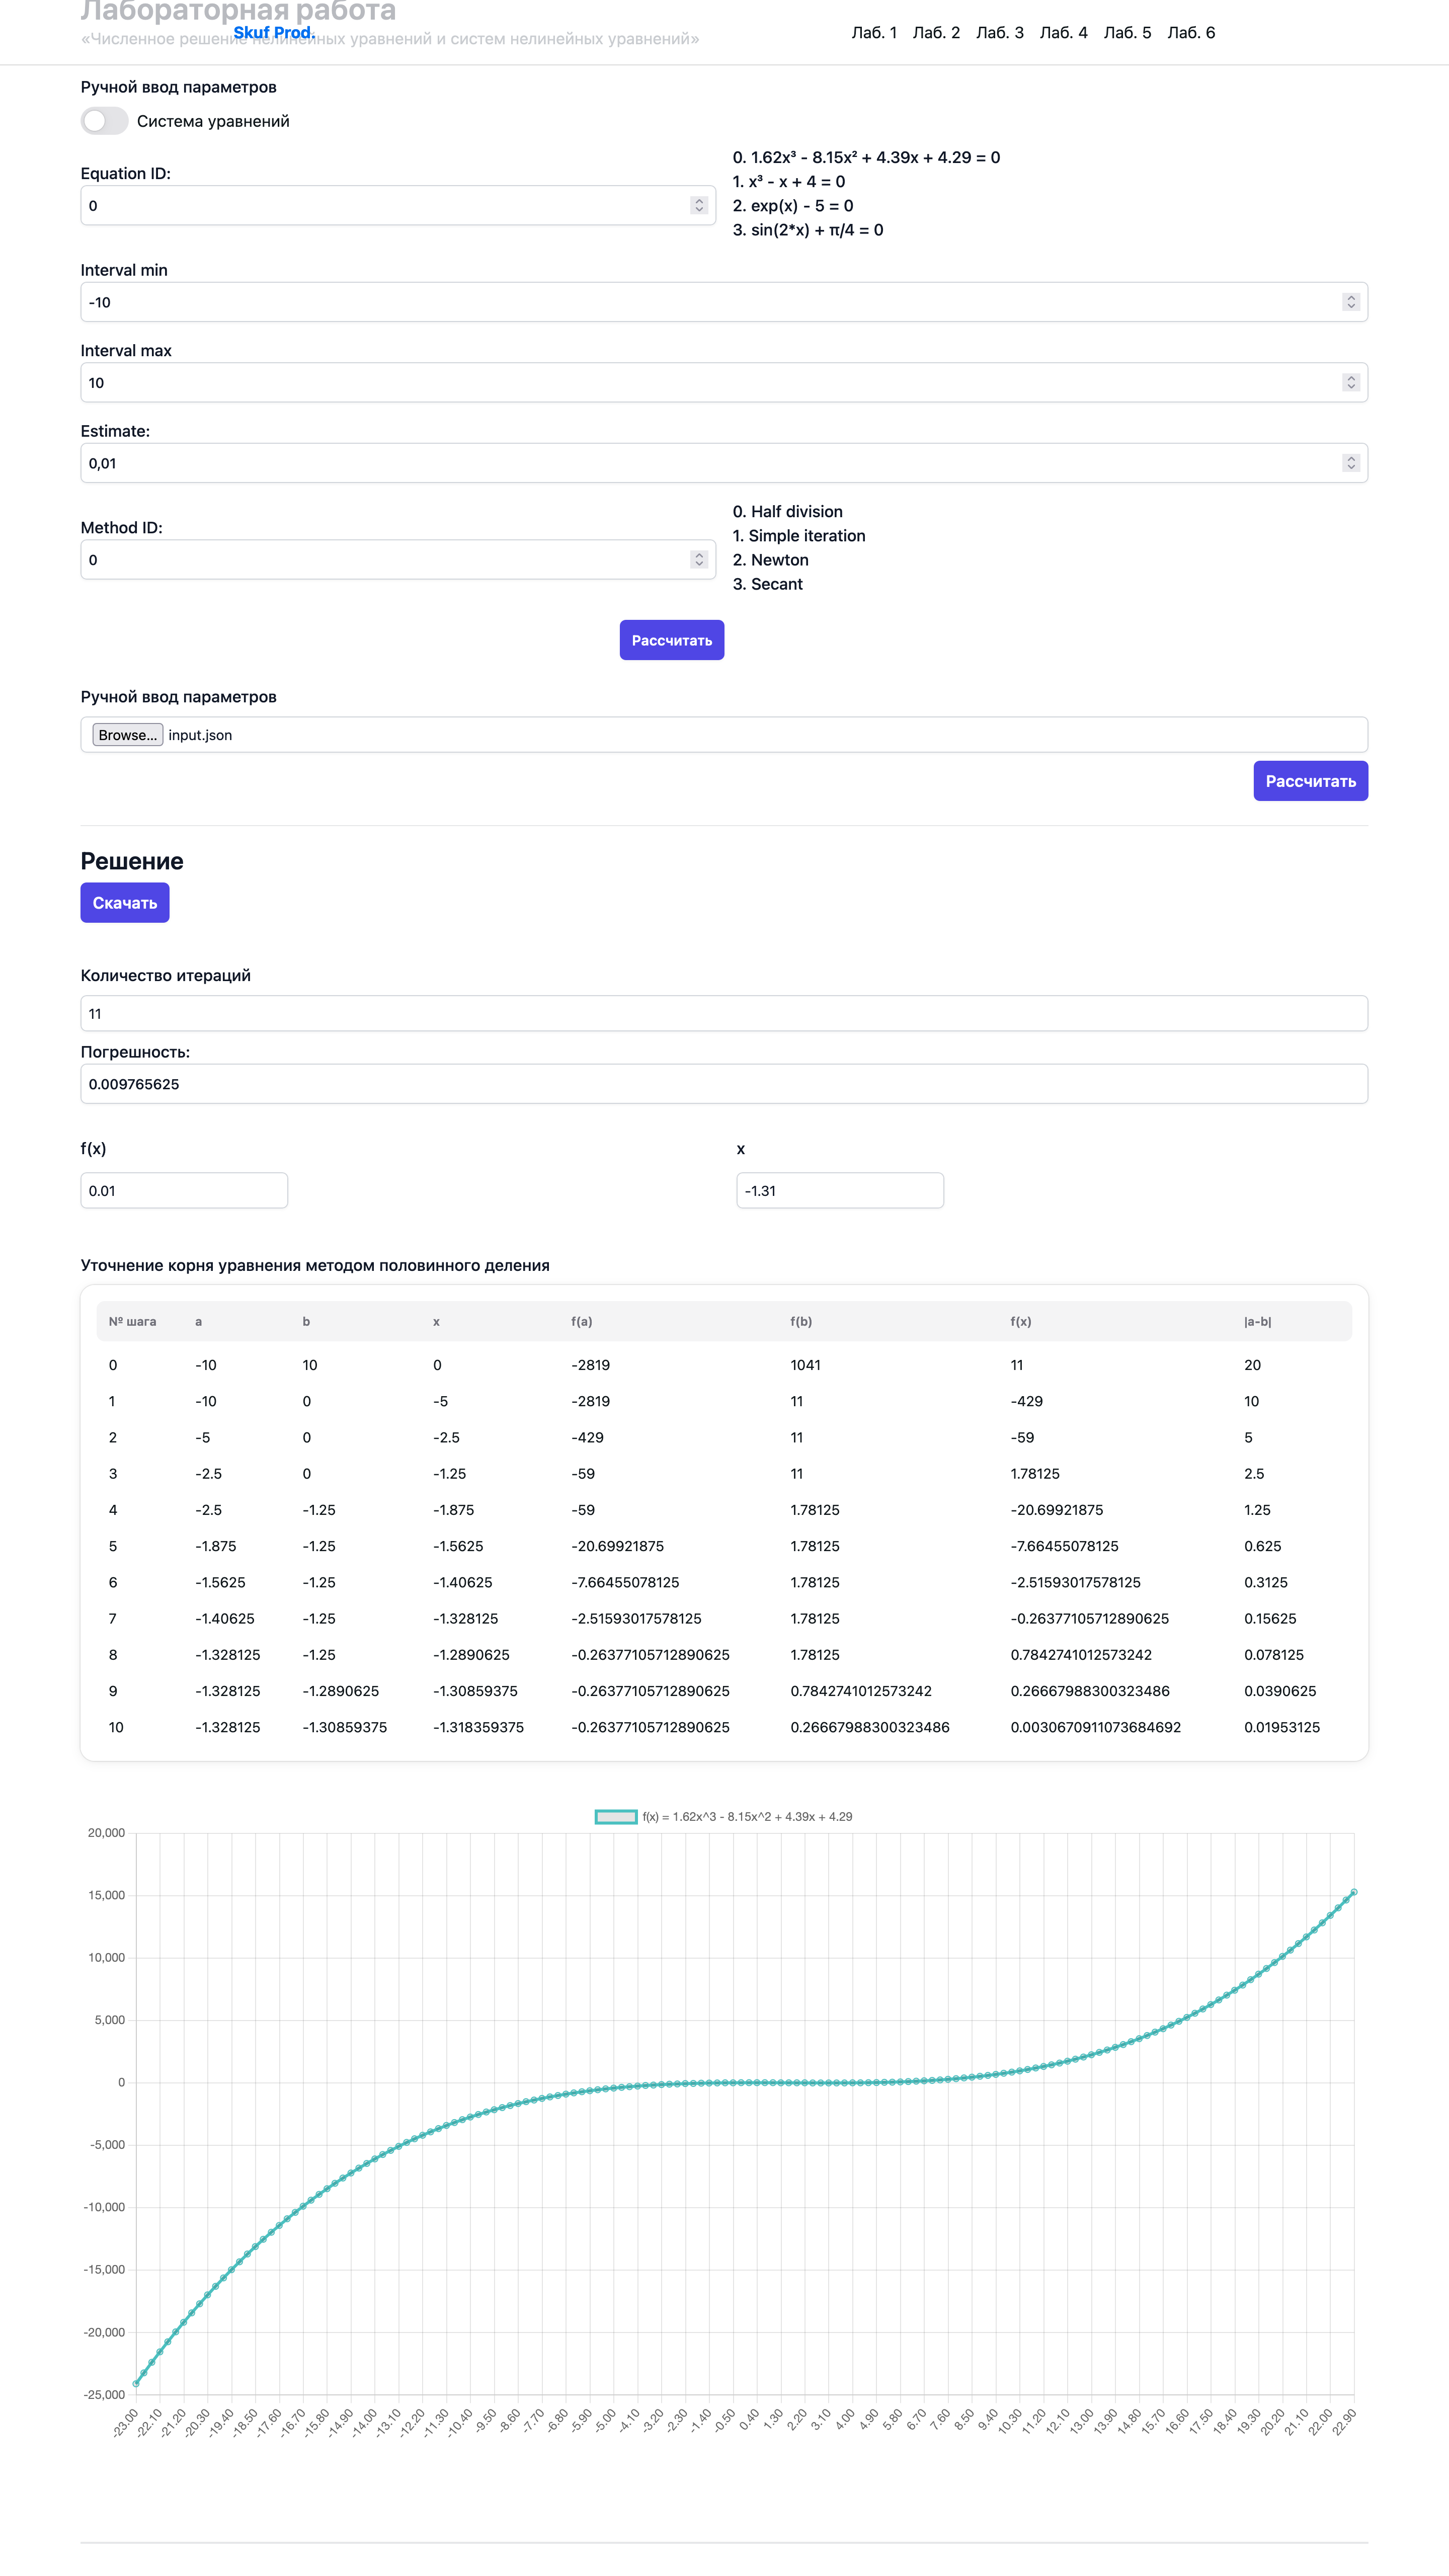
\includegraphics[scale=0.1]{SS2.png}
                        \caption{\small \sl UI 2}  
                  \end{center}  
            \end{figure}
            \begin{figure}[H] 
                  \begin{center}  
                        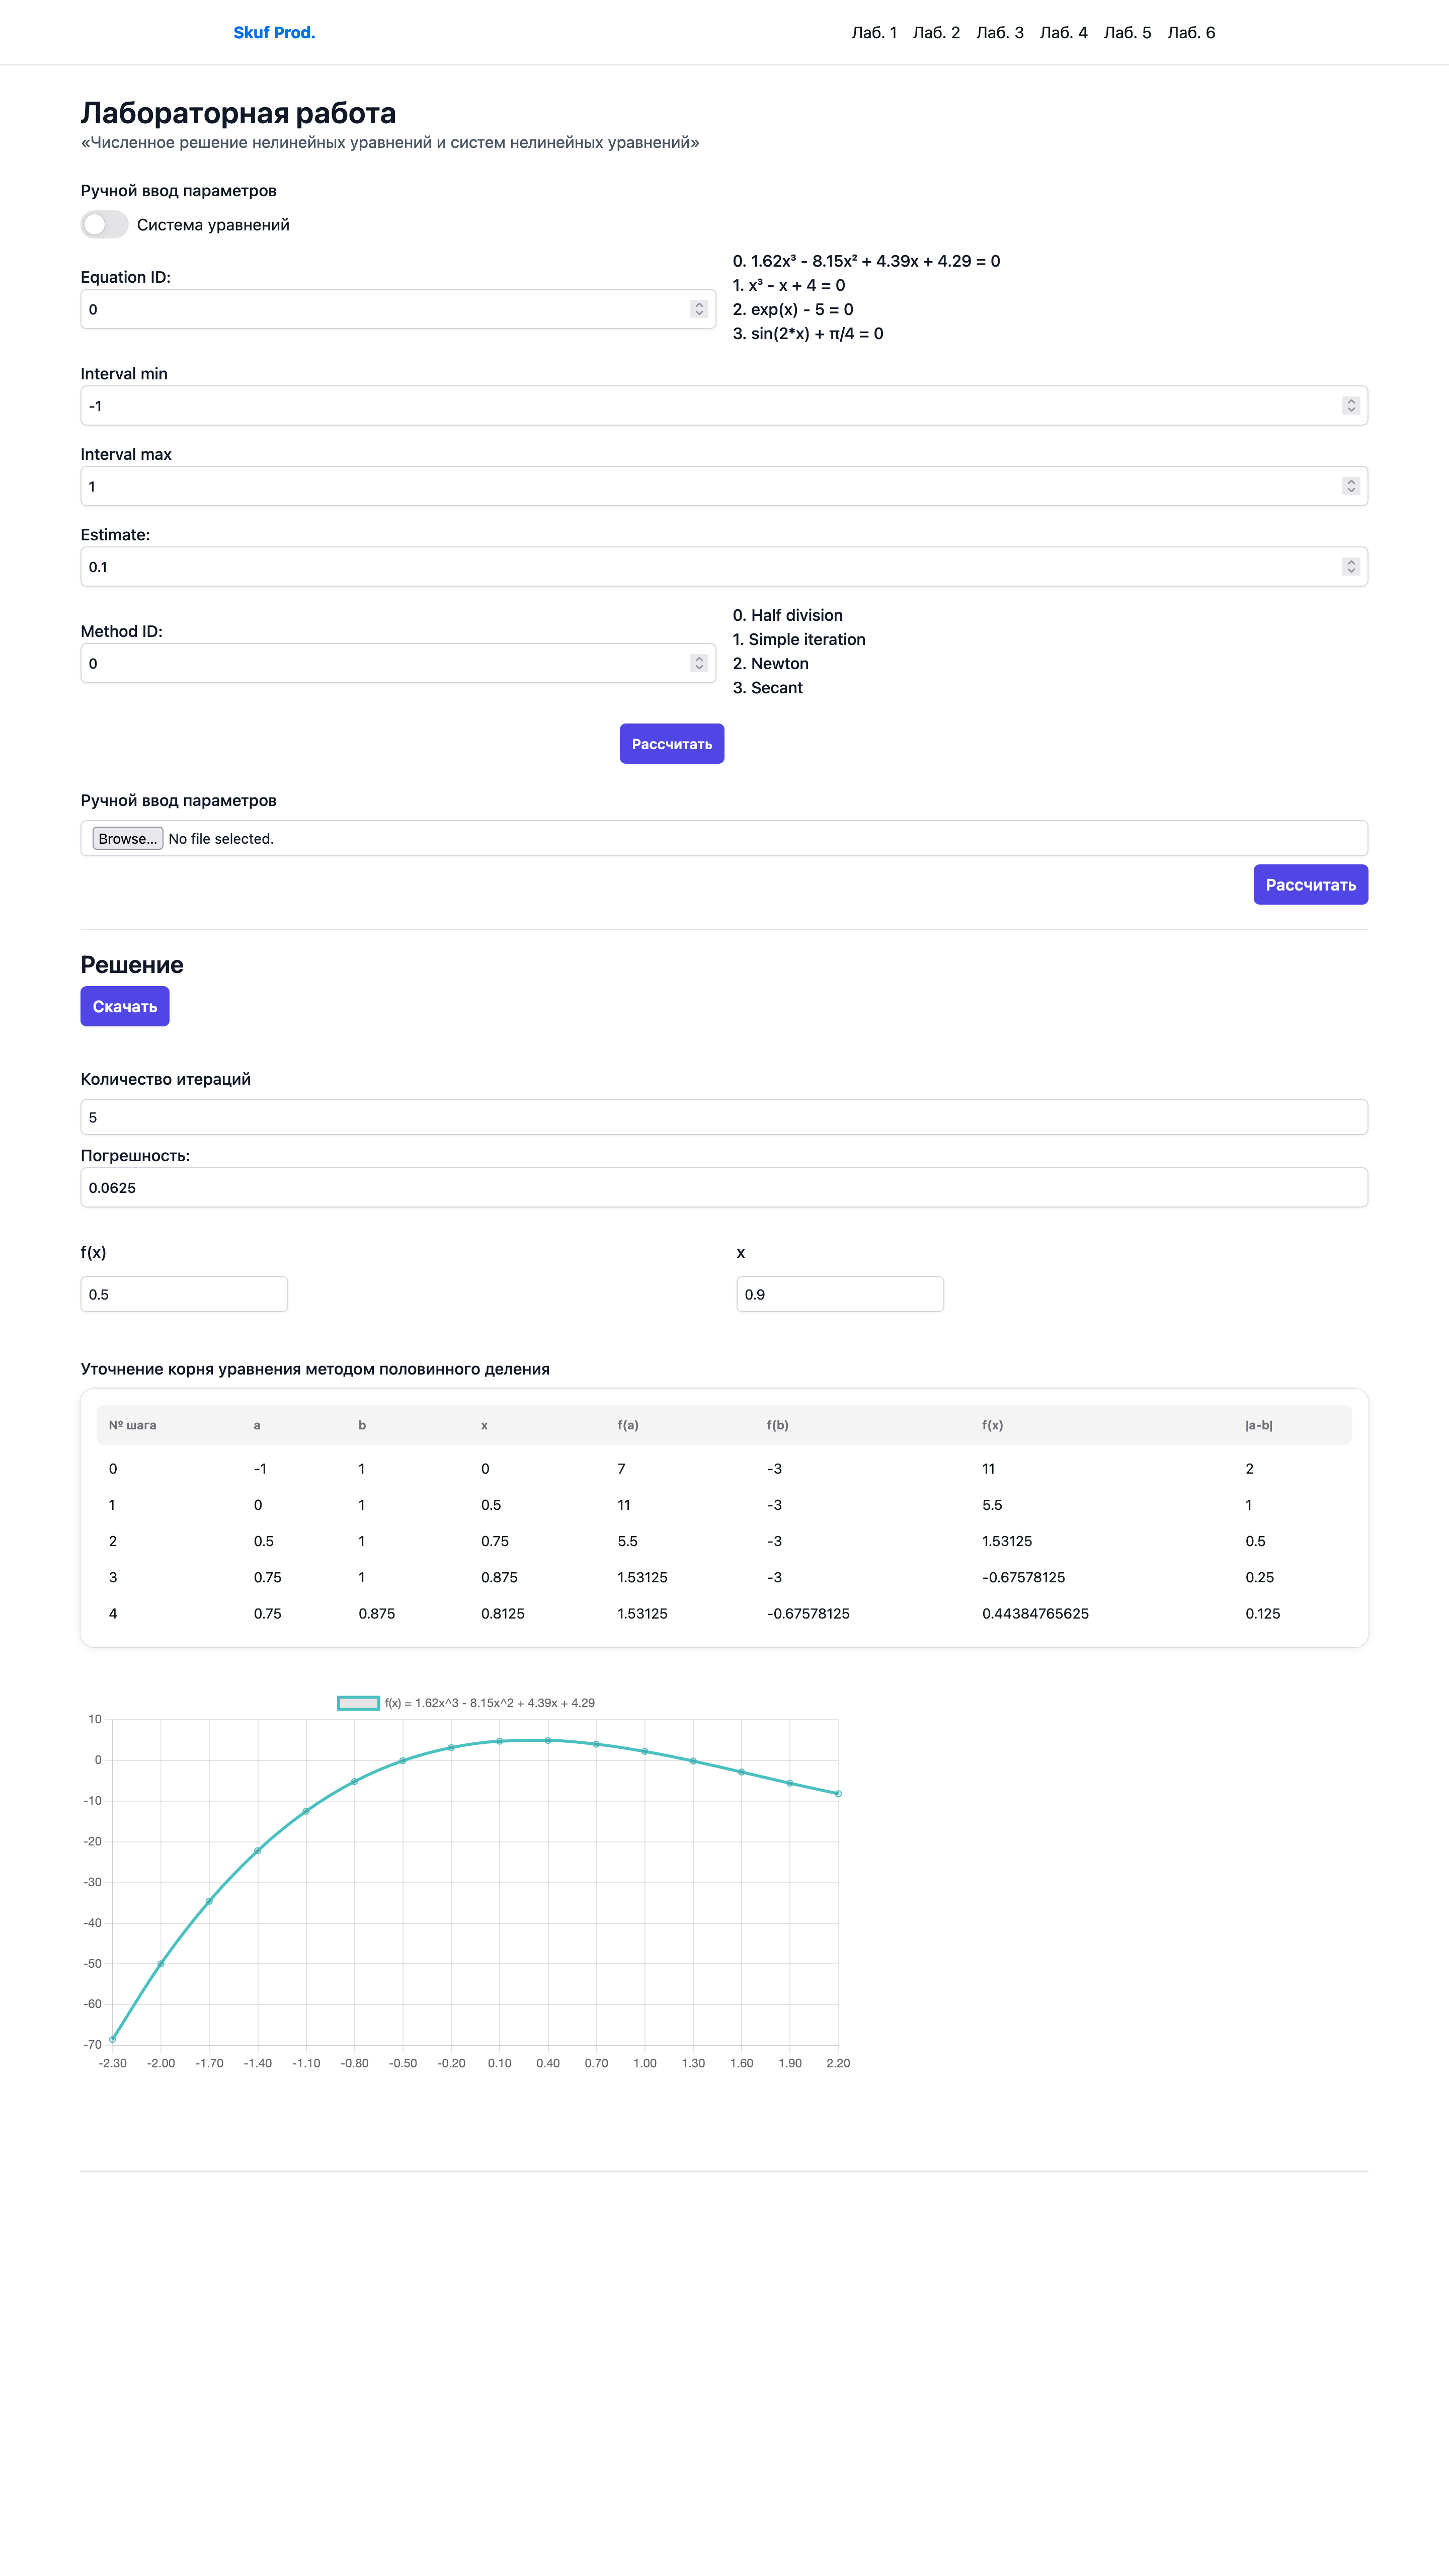
\includegraphics[scale=0.1]{SS3.png}
                        \caption{\small \sl UI 3}  
                  \end{center}  
            \end{figure}
      
\section{Заключение}
      В ходе выполнения данной ЛР я ознакомился с основыми методами решения нелинейных уравнений и систем нелинейных уравнений. Вообще с кайфом написал 2к строк кода

\begin{thebibliography}{9}
    \bibitem{Методичка}Слайды с лекций (2023). // Кафедра информатики и вычислительной техники -- Малышева Татьяна Алексеевна, к.т.н., доцент.
\end{thebibliography} 

\end{document}
